% =====================================================================
%  Script Matters: Measuring Latin-Script Banglish Robustness in
%  Bangla LLMs  —  B.Sc. Thesis Defense Presentation
%  Munim Thahmid (2005097) · Supervisor: Dr. Sadia Sharmin · BUET CSE
%  Compile with:  lualatex main.tex   (twice)
% =====================================================================
\documentclass[aspectratio=169,10pt]{beamer}

\usepackage{fontspec}
\usepackage{tikz}
\usetikzlibrary{positioning,arrows.meta,calc,shapes.misc}
\usepackage{pgfplots}
\pgfplotsset{compat=1.18}
\usepackage{booktabs}
\usepackage{colortbl}
\usepackage{amssymb}

% ---------------------------------------------------------------------
% Fonts
% ---------------------------------------------------------------------
\setsansfont{Noto Sans}
\setmonofont{DejaVu Sans Mono}[Scale=0.86]
\newfontfamily\bn{Noto Sans Bengali}[Renderer=HarfBuzz,Script=Bengali]
\newfontfamily\bnb{Noto Sans Bengali}[Renderer=HarfBuzz,Script=Bengali,UprightFont={* Bold}]

% ---------------------------------------------------------------------
% Palette  (mirrors the thesis figures: teal Bangla / coral Banglish /
% slate English)
% ---------------------------------------------------------------------
\definecolor{cInk}{HTML}{16242F}      % near-black text
\definecolor{cAccent}{HTML}{0F4C5C}   % deep teal (structure)
\definecolor{cBangla}{HTML}{2A9D8F}   % teal       — Bangla
\definecolor{cBanglish}{HTML}{E76F51} % coral      — Banglish
\definecolor{cEnglish}{HTML}{4A6FA5}  % slate blue — English
\definecolor{cMuted}{HTML}{64748B}    % gray
\definecolor{cBg}{HTML}{F2F5F7}       % card background
\definecolor{cGood}{HTML}{2F9E44}
\definecolor{cBad}{HTML}{D7263D}
\definecolor{cWarn}{HTML}{E8A50C}
\definecolor{cHard}{HTML}{7A8691}
\definecolor{cBoth}{HTML}{7E5AA2}

% ---------------------------------------------------------------------
% Beamer look: flat, white, thin rules
% ---------------------------------------------------------------------
\setbeamercolor{normal text}{fg=cInk}
\setbeamercolor{structure}{fg=cAccent}
\setbeamercolor{alerted text}{fg=cBanglish}
\setbeamercolor{itemize item}{fg=cAccent}
\setbeamercolor{itemize subitem}{fg=cMuted}
\setbeamertemplate{itemize item}{\raisebox{2pt}{\rule{4.5pt}{4.5pt}}}
\setbeamertemplate{itemize subitem}{--}
\setbeamertemplate{navigation symbols}{}
\setbeamersize{text margin left=0.85cm,text margin right=0.85cm}
\setbeamertemplate{frametitle}{%
  \vspace*{0.42cm}%
  {\fontsize{6.5}{8}\selectfont\bfseries\color{cMuted}%
    \MakeUppercase{\insertsection}\par}%
  \vspace*{1.5pt}%
  {\fontsize{15.5}{18}\selectfont\bfseries\color{cInk}\insertframetitle\par}%
  \vspace*{2.5pt}%
  {\color{cBanglish}\rule{1.05cm}{2.2pt}}\vspace*{0.5pt}%
}
\setbeamertemplate{footline}{%
  \hbox to \paperwidth{\hspace*{0.85cm}%
    {\fontsize{5.5}{6}\selectfont\color{cMuted}%
      Script Matters: Latin-Script Banglish Robustness in Bangla LLMs%
      \hfill Munim Thahmid · 2005097%
      \hfill\insertframenumber\,/\,\inserttotalframenumber}%
    \hspace*{0.85cm}}\vspace*{7pt}%
}

% ---------------------------------------------------------------------
% Helpers
% ---------------------------------------------------------------------
\newcommand{\cmark}{\textcolor{cGood}{\checkmark}}
\newcommand{\xmark}{\textcolor{cBad}{$\times$}}
\newcommand{\pmark}{\textcolor{cWarn}{$\sim$}}
\newcommand{\kicker}[1]{{\fontsize{6.5}{8}\selectfont\bfseries\color{cMuted}\MakeUppercase{#1}\par}}
% \scard{width}{border color}{title}{body}
\newcommand{\scard}[4]{%
  \begin{tikzpicture}
    \node[draw=#2,fill=#2!7,rounded corners=5pt,line width=1.1pt,
          text width=#1,inner sep=7pt,align=left]{%
      {\fontsize{8}{10}\selectfont\bfseries\color{#2!60!cInk}#3\par}%
      \vspace*{2.5pt}%
      {\fontsize{8}{10.5}\selectfont #4\par}};
  \end{tikzpicture}}

\title{Script Matters}
\author{Munim Thahmid}

\begin{document}

% =====================================================================
% 1 · TITLE
% =====================================================================
\begin{frame}[plain]
  \begin{tikzpicture}[remember picture,overlay]
    \fill[cInk] (current page.north west) rectangle (current page.south east);
    \fill[cBangla]   ([yshift=-0.0cm]current page.north west) rectangle ([yshift=-0.14cm,xshift=5.33cm]current page.north west);
    \fill[cBanglish] ([xshift=5.33cm]current page.north west) rectangle ([yshift=-0.14cm,xshift=10.67cm]current page.north west);
    \fill[cEnglish]  ([xshift=10.67cm]current page.north west) rectangle ([yshift=-0.14cm]current page.north east);
    \node[anchor=west,text width=13.5cm] at ([xshift=0.95cm,yshift=1.45cm]current page.west) {%
      {\fontsize{7.5}{9}\selectfont\bfseries\color{cBanglish}\MakeUppercase{B.Sc.\ in CSE — Thesis Defense}\par}
      \vspace*{8pt}
      {\fontsize{25}{29}\selectfont\bfseries\color{white}Script Matters\par}
      \vspace*{5pt}
      {\fontsize{12.5}{16}\selectfont\color{white!85!cInk}Measuring Latin-Script \textcolor{cBanglish}{Banglish} Robustness in Bangla LLMs\par}
      \vspace*{14pt}
      {\fontsize{8.5}{12}\selectfont\color{white!75!cInk}%
        {\bn আলো} \; \textcolor{cMuted}{·} \; \textit{alo} \; \textcolor{cMuted}{·} \; light
        --- same word, three scripts\par}
    };
    \node[anchor=south west,text width=6.6cm] at ([xshift=0.95cm,yshift=0.85cm]current page.south west) {%
      {\fontsize{8}{11}\selectfont\color{white!60!cInk}\bfseries Submitted by\par}
      {\fontsize{9.5}{13}\selectfont\color{white}Munim Thahmid \,·\, 2005097\par}};
    \node[anchor=south west,text width=7.2cm] at ([xshift=8.30cm,yshift=0.85cm]current page.south west) {%
      {\fontsize{8}{11}\selectfont\color{white!60!cInk}\bfseries Supervised by\par}
      {\fontsize{9.5}{13}\selectfont\color{white}Dr.\ Sadia Sharmin\par}
      {\fontsize{7.5}{10}\selectfont\color{white!60!cInk}Department of CSE, BUET \,·\, June 2026\par}};
  \end{tikzpicture}
\end{frame}

% =====================================================================
\section{Motivation}
% =====================================================================

% 2 · ONE QUESTION, THREE SCRIPTS
\begin{frame}{One question, three ways to type it}
  \vspace{2pt}
  A Bangladeshi student asks a model the \textbf{same science question}.
  The gold answer never changes --- only the \textbf{orthography} does.
  \vspace{8pt}
  \begin{center}
  \begin{tikzpicture}
    \node[draw=cBangla,fill=cBangla!7,rounded corners=6pt,line width=1.2pt,
          text width=3.65cm,inner sep=8pt,minimum height=2.25cm] (a) at (0,0) {%
      {\fontsize{7}{9}\selectfont\bfseries\color{cBangla!60!cInk}\MakeUppercase{Bangla (native script)}\par}\vspace*{4pt}
      {\bn\fontsize{9.5}{14}\selectfont সালোকসংশ্লেষণ কোথায় ঘটে?\par}};
    \node[draw=cBanglish,fill=cBanglish!7,rounded corners=6pt,line width=1.2pt,
          text width=3.65cm,inner sep=8pt,minimum height=2.25cm,right=0.45cm of a] (b) {%
      {\fontsize{7}{9}\selectfont\bfseries\color{cBanglish!70!cInk}\MakeUppercase{Banglish (Latin script)}\par}\vspace*{4pt}
      {\fontsize{9.5}{13}\selectfont\itshape Salokshongshleshon kothay ghote?\par}};
    \node[draw=cEnglish,fill=cEnglish!7,rounded corners=6pt,line width=1.2pt,
          text width=3.65cm,inner sep=8pt,minimum height=2.25cm,right=0.45cm of b] (c) {%
      {\fontsize{7}{9}\selectfont\bfseries\color{cEnglish!70!cInk}\MakeUppercase{English}\par}\vspace*{4pt}
      {\fontsize{9.5}{13}\selectfont Where does photosynthesis take place?\par}};
    \node[below=0.32cm of b,text width=12.6cm,align=center] {%
      {\fontsize{9}{12}\selectfont Same task \,·\, same item id \,·\, \textbf{same gold answer}\par}};
  \end{tikzpicture}
  \end{center}
  \vspace{4pt}
  \begin{itemize}
    \item Banglish is how Bangla actually reaches models in messaging, comments,
          search, and informal learning --- Latin keyboards are simply convenient.
    \item A model may answer one version and \alert{fail another}, even though
          the answer has not changed.
  \end{itemize}
\end{frame}

% 3 · THE HIDDEN ACCESS GAP
\begin{frame}{Banglish is everywhere --- but benchmarks don't isolate it}
  \vspace{2pt}
  \begin{columns}[T]
    \column{0.52\textwidth}
      \kicker{What prior datasets establish}
      \vspace{3pt}
      \begin{itemize}
        \item \textbf{BanglaTLit}: romanized Bangla is widespread and highly
              \textbf{spelling-variable} (a back-transliteration problem of its own)
        \item \textbf{BanglishRev, BAN-TH, BnSentMix, MixSarc}: Banglish \& code-mixed
              text fill reviews, social media, sentiment, hate-speech data
        \item \textbf{Bhasha-abhijnaanam}: romanized Indic LID is treated as an
              \emph{infrastructure} problem
      \end{itemize}
      \vspace{4pt}
      {\fontsize{9}{12}\selectfont So Banglish is a \textbf{real access path} for
       millions of users --- not an academic curiosity.\par}
    \column{0.44\textwidth}
      \kicker{What gets evaluated today}
      \vspace{3pt}
      \begin{center}
      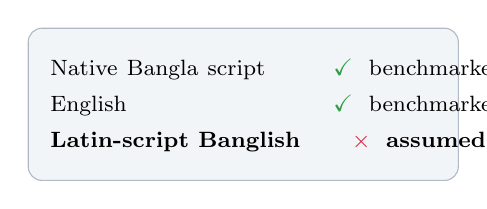
\begin{tikzpicture}
        \node[draw=cMuted!50,fill=cBg,rounded corners=5pt,inner sep=8pt,text width=4.9cm]{%
          {\fontsize{8.5}{13}\selectfont
            \begin{tabular}{@{}lc@{}}
              Native Bangla script & \cmark\; benchmarked\\
              English              & \cmark\; benchmarked\\
              \textbf{Latin-script Banglish} & \xmark\; \textbf{assumed}\\
            \end{tabular}\par}};
      \end{tikzpicture}
      \end{center}
      \vspace{6pt}
      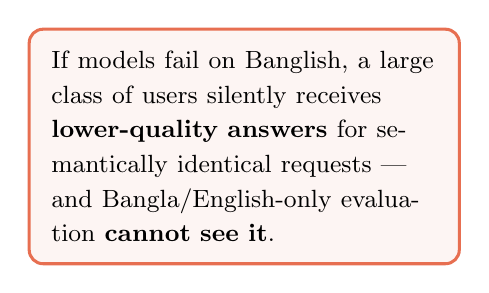
\begin{tikzpicture}
        \node[draw=cBanglish,fill=cBanglish!7,rounded corners=5pt,inner sep=8pt,
              line width=1.1pt,text width=4.9cm]{%
          {\fontsize{9}{12.5}\selectfont If models fail on Banglish, a large class of
           users silently receives \textbf{lower-quality answers} for semantically
           identical requests --- and Bangla/English-only evaluation
           \textbf{cannot see it}.\par}};
      \end{tikzpicture}
  \end{columns}
\end{frame}

% =====================================================================
\section{Research Question}
% =====================================================================

% 4 · RESEARCH QUESTION (dark statement slide)
\begin{frame}[plain]
  \begin{tikzpicture}[remember picture,overlay]
    \fill[cInk] (current page.north west) rectangle (current page.south east);
    \node[anchor=west,text width=13.6cm] at ([xshift=0.95cm,yshift=0.95cm]current page.west) {%
      {\fontsize{7.5}{9}\selectfont\bfseries\color{cBanglish}\MakeUppercase{Research question}\par}
      \vspace*{10pt}
      {\fontsize{17}{23}\selectfont\bfseries\color{white}%
        If the task and the gold answer are held fixed,\par
        does changing the script to Latin-script Banglish\par
        change model reliability?\par}
      \vspace*{14pt}
      {\fontsize{9.5}{14}\selectfont\color{white!70!cInk}%
        This is \textbf{\textcolor{white}{not}} ``is Bangla hard for LLMs?'' ---
        it frames Banglish as an \textbf{\textcolor{cBanglish}{orthographic access problem}}:
        script choice as a measurable robustness variable.\par}
    };
    \node[anchor=south west] at ([xshift=0.95cm,yshift=0.75cm]current page.south west){%
      \begin{tikzpicture}[every node/.style={rounded corners=4pt,inner sep=6pt,
                          font=\fontsize{8}{10}\selectfont\bfseries}]
        \node[fill=cBangla!25,text=cBangla!20!white] (p1) {1 · Evaluation must be \emph{paired}};
        \node[fill=cBanglish!25,text=cBanglish!15!white,right=0.35cm of p1] (p2) {2 · Banglish must be \emph{human-audited}};
        \node[fill=cEnglish!25,text=cEnglish!15!white,right=0.35cm of p2] (p3) {3 · Strong models are a \emph{boundary test}};
      \end{tikzpicture}};
  \end{tikzpicture}
\end{frame}

% =====================================================================
\section{Related Work}
% =====================================================================

% 5 · GAP TABLE
\begin{frame}{The missing piece in a crowded Bengali-evaluation landscape}
  \vspace{2pt}
  Bengali LLM evaluation is active --- BEnQA, BanglaMATH, BanglaQuAD, BnMMLU, BLUCK,
  NCTB-QA, BNLI, safety \& social benchmarks. \textbf{None isolates script while
  holding the task and answer fixed.} Closest neighbors:
  \vspace{6pt}
  \begin{center}
  {\fontsize{8.5}{12}\selectfont
  \renewcommand{\arraystretch}{1.25}
  \begin{tabular}{@{}lccccc@{}}
    \toprule
    \textbf{Work} & \textbf{Paired} & \textbf{Human-rev.} & \textbf{Downstream} & \textbf{Mitigation} & \textbf{Scale}\\
                  & \textbf{items}  & \textbf{romanization} & \textbf{QA/math} & \textbf{study} & \textbf{extension}\\
    \midrule
    Transliteration perturbations \,{\scriptsize(BLP 2025)} & \pmark\;partial & \xmark & \xmark & \xmark & \xmark\\
    Script-gap triage \,{\scriptsize(clinical, 2025)}       & \cmark          & \xmark & \xmark & \xmark & \xmark\\
    Romanized Nepali \,{\scriptsize(2026)}                  & \pmark\;partial & \xmark & \xmark & \cmark & \xmark\\
    \rowcolor{cBangla!12}
    \textbf{This thesis} & \cmark & \cmark & \cmark & \cmark & \cmark\\
    \bottomrule
  \end{tabular}\par}
  \end{center}
  \vspace{6pt}
  \begin{itemize}
    \item Prior work perturbs words/sentences or evaluates one classification task;
          none combines \textbf{gold-answer tasks + human-reviewed romanization +
          multi-model measurement + mitigation + scale} under one protocol.
  \end{itemize}
\end{frame}

% 6 · CONTRIBUTIONS
\begin{frame}{Contributions at a glance}
  \vspace{3pt}
  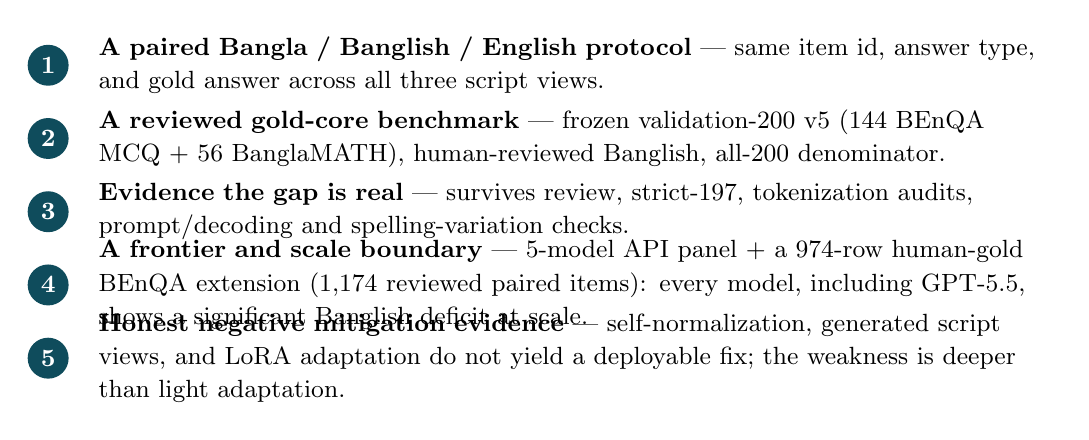
\begin{tikzpicture}[
      num/.style={circle,fill=cAccent,text=white,font=\bfseries\fontsize{9}{9}\selectfont,
                  minimum size=0.52cm,inner sep=0pt},
      lab/.style={anchor=west,text width=12.1cm,font=\fontsize{9}{12}\selectfont}]
    \node[num] (n1) at (0,0)     {1};
    \node[lab,right=0.25cm of n1]{\textbf{A paired Bangla / Banglish / English protocol} ---
      same item id, answer type, and gold answer across all three script views.};
    \node[num] (n2) at (0,-0.93) {2};
    \node[lab,right=0.25cm of n2]{\textbf{A reviewed gold-core benchmark} --- frozen
      validation-200 v5 (144 BEnQA MCQ + 56 BanglaMATH), human-reviewed Banglish, all-200 denominator.};
    \node[num] (n3) at (0,-1.86) {3};
    \node[lab,right=0.25cm of n3]{\textbf{Evidence the gap is real} --- survives review,
      strict-197, tokenization audits, prompt/decoding and spelling-variation checks.};
    \node[num] (n4) at (0,-2.79) {4};
    \node[lab,right=0.25cm of n4]{\textbf{A frontier and scale boundary} --- 5-model API panel
      + a 974-row human-gold BEnQA extension (1{,}174 reviewed paired items): every model,
      including GPT-5.5, shows a significant Banglish deficit at scale.};
    \node[num] (n5) at (0,-3.72) {5};
    \node[lab,right=0.25cm of n5]{\textbf{Honest negative mitigation evidence} ---
      self-normalization, generated script views, and LoRA adaptation do not yield a
      deployable fix; the weakness is deeper than light adaptation.};
  \end{tikzpicture}
\end{frame}

% =====================================================================
\section{Methodology}
% =====================================================================

% 7 · PIPELINE
\begin{frame}{Benchmark construction: two human-reviewed tracks, one protocol}
  \vspace{4pt}
  \begin{center}
  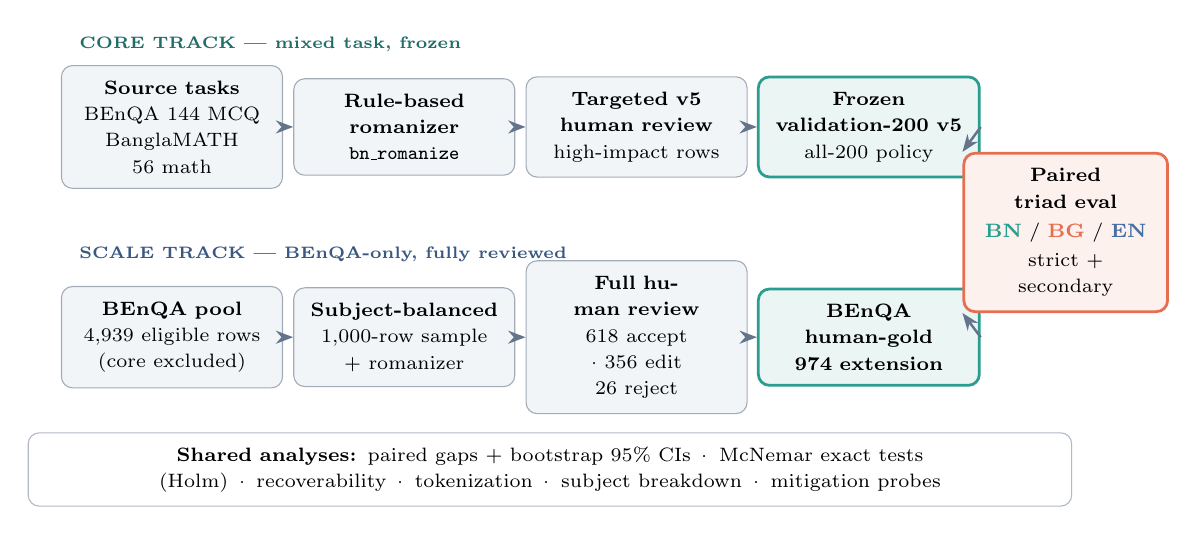
\begin{tikzpicture}[
      box/.style={draw=cMuted!60,fill=cBg,rounded corners=4pt,inner sep=5.5pt,
                  text width=2.42cm,align=center,font=\fontsize{7.5}{9.5}\selectfont},
      gbox/.style={box,draw=cBangla,fill=cBangla!10,line width=1pt},
      ebox/.style={box,draw=cBanglish,fill=cBanglish!10,line width=1pt,text width=2.2cm},
      arr/.style={-{Stealth[length=2.2mm]},cMuted,line width=0.9pt},
      lab/.style={font=\fontsize{6.5}{8}\selectfont\bfseries\color{cMuted}}]
    % top track
    \node[lab,anchor=west] at (-0.1,1.05) {\textcolor{cBangla!60!cInk}{CORE TRACK — mixed task, frozen}};
    \node[box] (t1) at (1.2,0)  {\textbf{Source tasks}\\ BEnQA 144 MCQ\\ BanglaMATH 56 math};
    \node[box] (t2) at (4.15,0) {\textbf{Rule-based}\\ \textbf{romanizer}\\ \texttt{bn\_romanize}};
    \node[box] (t3) at (7.1,0)  {\textbf{Targeted v5}\\ \textbf{human review}\\ high-impact rows};
    \node[gbox] (t4) at (10.05,0) {\textbf{Frozen}\\ \textbf{validation-200 v5}\\ all-200 policy};
    \draw[arr] (t1) -- (t2); \draw[arr] (t2) -- (t3); \draw[arr] (t3) -- (t4);
    % bottom track
    \node[lab,anchor=west] at (-0.1,-1.62) {\textcolor{cEnglish!70!cInk}{SCALE TRACK — BEnQA-only, fully reviewed}};
    \node[box] (b1) at (1.2,-2.67)  {\textbf{BEnQA pool}\\ 4{,}939 eligible rows\\ (core excluded)};
    \node[box] (b2) at (4.15,-2.67) {\textbf{Subject-balanced}\\ 1{,}000-row sample\\ + romanizer};
    \node[box] (b3) at (7.1,-2.67)  {\textbf{Full human review}\\ 618 accept · 356 edit\\ 26 reject};
    \node[gbox] (b4) at (10.05,-2.67) {\textbf{BEnQA human-gold}\\ \textbf{974 extension}};
    \draw[arr] (b1) -- (b2); \draw[arr] (b2) -- (b3); \draw[arr] (b3) -- (b4);
    % eval node
    \node[ebox,minimum height=1.5cm] (ev) at (12.55,-1.34) {\textbf{Paired triad eval}\\[1pt]
      {\color{cBangla}\textbf{BN}} / {\color{cBanglish}\textbf{BG}} / {\color{cEnglish}\textbf{EN}}\\[1pt]
      strict + secondary};
    \draw[arr] (t4.east) -- (ev.north west);
    \draw[arr] (b4.east) -- (ev.south west);
    % analyses bar
    \node[draw=cMuted!50,fill=white,rounded corners=4pt,inner sep=5pt,text width=12.9cm,
          align=center,font=\fontsize{7.5}{9.5}\selectfont] at (6.0,-4.35)
      {\textbf{Shared analyses:} paired gaps + bootstrap 95\% CIs \,·\, McNemar exact tests (Holm)
       \,·\, recoverability \,·\, tokenization \,·\, subject breakdown \,·\, mitigation probes};
  \end{tikzpicture}
  \end{center}
  \vspace{2pt}
  {\fontsize{8.5}{11}\selectfont Frozen \emph{before} outcomes are seen; three flagged
   source-quality rows tracked under a separate strict-197 sensitivity view.\par}
\end{frame}

% 8 · TRIAD PROTOCOL
\begin{frame}{The paired triad: script is the only variable}
  \vspace{2pt}
  \begin{columns}[T]
    \column{0.56\textwidth}
      \kicker{One item, three views}
      \vspace{4pt}
      \begin{tikzpicture}[every node/.style={rounded corners=5pt,inner sep=6.5pt,text width=5.6cm}]
        \node[draw=cBangla,fill=cBangla!7,line width=1pt] (v1) at (0,0) {%
          {\fontsize{7.5}{10}\selectfont {\color{cBangla!60!cInk}\textbf{BN}}\;
           {\bn তামার রোধকত্ব কত?} \hfill {\color=cMuted}\par}};
        \node[draw=cBanglish,fill=cBanglish!7,line width=1pt,below=0.22cm of v1] (v2) {%
          {\fontsize{7.5}{10}\selectfont {\color{cBanglish!70!cInk}\textbf{BG}}\;
           \textit{Tamar rodhokotto koto?}\par}};
        \node[draw=cEnglish,fill=cEnglish!7,line width=1pt,below=0.22cm of v2] (v3) {%
          {\fontsize{7.5}{10}\selectfont {\color{cEnglish!70!cInk}\textbf{EN}}\;
           What is the resistivity of copper?\par}};
        \node[draw=cMuted!50,fill=cBg,below=0.26cm of v3,text width=5.6cm] (gold) {%
          {\fontsize{7.5}{10}\selectfont\textbf{Gold answer (fixed):} option \textbf{C}
           \hfill answer-only prompt\par}};
      \end{tikzpicture}
    \column{0.42\textwidth}
      \kicker{Preserved invariants}
      \vspace{3pt}
      {\fontsize{9}{13}\selectfont
      \begin{itemize}
        \item item id \,·\, answer type \,·\, gold answer
        \item BEnQA $\to$ one letter A--D; BanglaMATH $\to$ short numeric answer
      \end{itemize}\par}
      \vspace{4pt}
      \kicker{Headline metric}
      \vspace{3pt}
      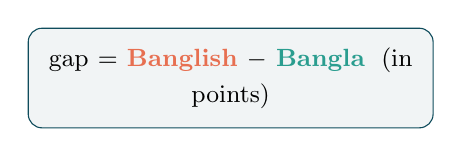
\begin{tikzpicture}
        \node[draw=cAccent,fill=cAccent!6,rounded corners=5pt,inner sep=7pt,text width=4.65cm]{%
          {\fontsize{9}{13}\selectfont\centering
            gap $=$ {\color{cBanglish}\textbf{Banglish}} $-$ {\color{cBangla}\textbf{Bangla}}
            \;(in points)\par}};
      \end{tikzpicture}
      \vspace{4pt}
      {\fontsize{8.5}{12}\selectfont A \emph{script gap} means the \textbf{same item}
       flips correctness when rewritten --- never that different questions were
       compared. English serves as a privileged semantic-check view.\par}
  \end{columns}
\end{frame}

% 9 · MODELS & SCORING
\begin{frame}{Models, scoring, and statistics}
  \vspace{2pt}
  \begin{columns}[T]
    \column{0.46\textwidth}
      \kicker{Open triad — reproducible core}
      \vspace{3pt}
      {\fontsize{9}{13}\selectfont
      \begin{itemize}
        \item Qwen2.5-3B-Instruct
        \item Qwen2.5-7B-Instruct (8-bit)
        \item Qwen3-4B-Instruct
        \item[] {\color{cMuted}\fontsize{8}{11}\selectfont + 4 extra Qwen sizes for the scaling study}
      \end{itemize}\par}
      \vspace{5pt}
      \kicker{Frontier / API panel — boundary test}
      \vspace{3pt}
      {\fontsize{9}{13}\selectfont
      \begin{itemize}
        \item Gemini 3.5 Flash \,·\, GPT-5.5 (low)
        \item Claude Sonnet 4.6 \,·\, DeepSeek V4 Flash
        \item Groq-hosted Llama 3.3 70B
      \end{itemize}\par}
    \column{0.50\textwidth}
      \kicker{Two scoring lenses}
      \vspace{3pt}
      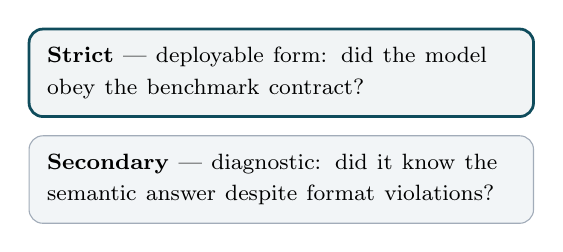
\begin{tikzpicture}[every node/.style={rounded corners=5pt,inner sep=6.5pt,text width=5.95cm}]
        \node[draw=cAccent,fill=cAccent!6,line width=1pt] (s1) {%
          {\fontsize{8.5}{11.5}\selectfont\textbf{Strict} --- deployable form: did the model
           obey the benchmark contract?\par}};
        \node[draw=cMuted!60,fill=cBg,below=0.22cm of s1] (s2) {%
          {\fontsize{8.5}{11.5}\selectfont\textbf{Secondary} --- diagnostic: did it know the
           semantic answer despite format violations?\par}};
      \end{tikzpicture}
      \vspace{5pt}
      \kicker{Statistics — paired by design}
      \vspace{3pt}
      {\fontsize{9}{13}\selectfont
      \begin{itemize}
        \item Paired bootstrap 95\% CIs on every gap
        \item \textbf{McNemar exact tests} on discordant pairs, Holm-corrected
        \item Same frozen prompt manifest \& parser for every model --- not a leaderboard
      \end{itemize}\par}
  \end{columns}
\end{frame}

% =====================================================================
\section{Main Results}
% =====================================================================

% 10 · MAIN RESULT
\begin{frame}{Reviewed Banglish is the weakest script view --- for every model}
  \vspace{2pt}
  \begin{columns}[T]
    \column{0.66\textwidth}
      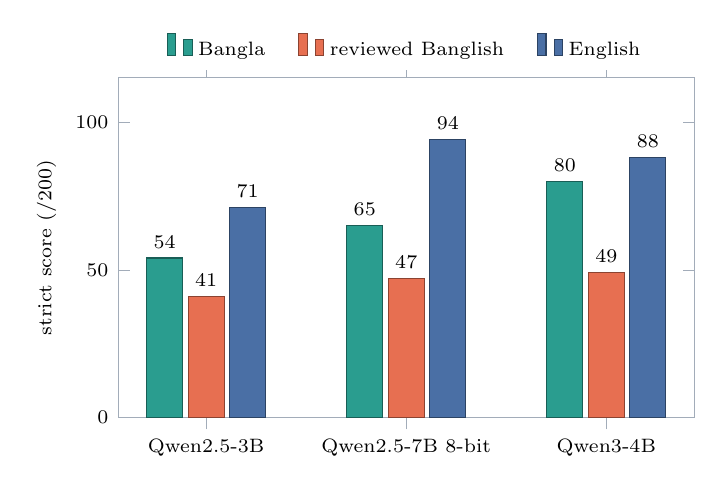
\begin{tikzpicture}
        \begin{axis}[
            ybar, bar width=13pt, width=8.9cm, height=5.9cm,
            ymin=0, ymax=115,
            symbolic x coords={Qwen2.5-3B, Qwen2.5-7B 8-bit, Qwen3-4B},
            xtick=data,
            x tick label style={font=\fontsize{7.5}{9}\selectfont},
            ytick={0,50,100},
            ylabel={strict score (/200)},
            y label style={font=\fontsize{7.5}{9}\selectfont},
            y tick label style={font=\fontsize{7.5}{9}\selectfont},
            enlarge x limits=0.22,
            axis line style={cMuted!60}, tick style={cMuted!60},
            nodes near coords,
            every node near coord/.append style={font=\fontsize{7}{8}\selectfont\bfseries},
            legend style={at={(0.5,1.02)},anchor=south,legend columns=3,
                          draw=none,font=\fontsize{7.5}{9}\selectfont,
                          /tikz/every even column/.append style={column sep=0.35cm}},
          ]
          \addplot[fill=cBangla,draw=cBangla!60!black]   coordinates {(Qwen2.5-3B,54) (Qwen2.5-7B 8-bit,65) (Qwen3-4B,80)};
          \addplot[fill=cBanglish,draw=cBanglish!60!black] coordinates {(Qwen2.5-3B,41) (Qwen2.5-7B 8-bit,47) (Qwen3-4B,49)};
          \addplot[fill=cEnglish,draw=cEnglish!60!black]  coordinates {(Qwen2.5-3B,71) (Qwen2.5-7B 8-bit,94) (Qwen3-4B,88)};
          \legend{Bangla, reviewed Banglish, English}
        \end{axis}
      \end{tikzpicture}
    \column{0.32\textwidth}
      \kicker{Frozen validation-200 v5}
      \vspace{4pt}
      {\fontsize{8.7}{12.5}\selectfont
      \begin{itemize}
        \item Banglish $-$ Bangla: \textbf{$-$6.5} / \textbf{$-$9.0} / \textbf{$-$15.5} pts
        \item Banglish $-$ English: $-$15 to $-$23.5 pts --- the same items \emph{are}
              answerable in another view
        \item BanglaMATH under Banglish: strict accuracy collapses to
              \textbf{0/56, 0/56, 2/56}
      \end{itemize}\par}
      \vspace{4pt}
      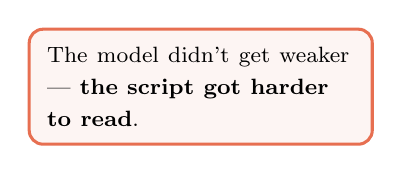
\begin{tikzpicture}
        \node[draw=cBanglish,fill=cBanglish!7,rounded corners=5pt,inner sep=6.5pt,
              line width=1.1pt,text width=3.9cm]{%
          {\fontsize{8.5}{11.5}\selectfont The model didn't get weaker ---
           \textbf{the script got harder to read}.\par}};
      \end{tikzpicture}
  \end{columns}
\end{frame}

% 11 · SIGNIFICANCE
\begin{frame}{The gap is statistically real, not noise}
  \vspace{2pt}
  \begin{columns}[T]
    \column{0.55\textwidth}
      \kicker{Banglish $-$ Bangla gap with paired bootstrap 95\% CI}
      \vspace{2pt}
      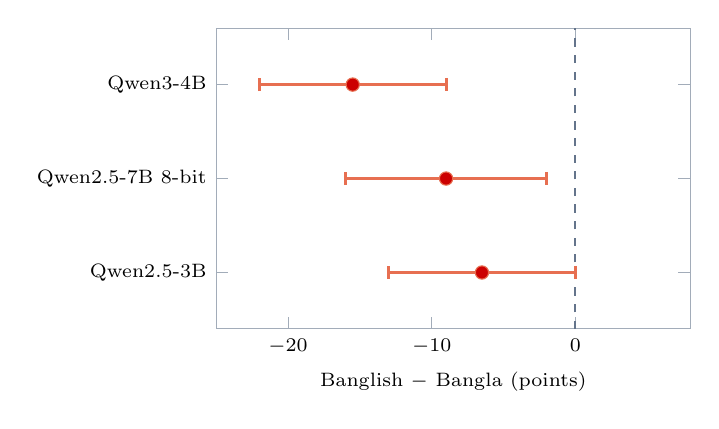
\begin{tikzpicture}
        \begin{axis}[
            width=7.6cm, height=5.4cm,
            xmin=-25, xmax=8,
            ytick={1,2,3},
            yticklabels={Qwen2.5-3B, Qwen2.5-7B 8-bit, Qwen3-4B},
            y tick label style={font=\fontsize{7.5}{9}\selectfont},
            x tick label style={font=\fontsize{7.5}{9}\selectfont},
            xlabel={Banglish $-$ Bangla (points)},
            x label style={font=\fontsize{7.5}{9}\selectfont},
            ymin=0.4, ymax=3.6,
            axis line style={cMuted!60}, tick style={cMuted!60},
          ]
          \addplot[cMuted,dashed,line width=0.8pt] coordinates {(0,0.4) (0,3.6)};
          \addplot+[only marks,mark=*,mark size=2.4pt,color=cBanglish,
                    error bars/.cd, x dir=both, x explicit,
                    error bar style={line width=1.1pt,color=cBanglish},
                    error mark options={rotate=90,mark size=2.4pt,line width=1.1pt}]
            coordinates {
              (-6.5,1)  +- (6.5,0)
              (-9.0,2)  +- (7.0,0)
              (-15.5,3) +- (6.5,0)
            };
        \end{axis}
      \end{tikzpicture}
    \column{0.43\textwidth}
      \kicker{McNemar exact tests (discordant pairs)}
      \vspace{4pt}
      {\fontsize{8.3}{11}\selectfont
      \renewcommand{\arraystretch}{1.3}
      \begin{tabular}{@{}lcccc@{}}
        \toprule
        \textbf{Model} & $b$ & $c$ & \textbf{OR} & \textbf{Holm $p$}\\
        \midrule
        Qwen2.5-3B      & 28 & 15 & 1.84 & 0.066\\
        Qwen2.5-7B 8-bit & 37 & 19 & 1.92 & \textbf{0.044}\\
        Qwen3-4B        & 39 &  8 & 4.65 & $\mathbf{<0.0001}$\\
        \bottomrule
      \end{tabular}\par}
      \vspace{4pt}
      {\fontsize{8.3}{11}\selectfont $b$ = Bangla-only correct \,·\, $c$ = Banglish-only
       correct. Tests use \emph{only} items that flip between scripts.\par}
      \vspace{5pt}
      {\fontsize{8.7}{12}\selectfont
      \begin{itemize}
        \item The marginal 3B result ($p{=}0.066$) becomes \textbf{significant
              ($p{=}0.024$) on the 974-row extension} --- sample size, not absence of effect
        \item Banglish vs English: $p \le 0.0001$ for \textbf{all three} models
      \end{itemize}\par}
  \end{columns}
\end{frame}

% =====================================================================
\section{Robustness Checks}
% =====================================================================

% 12 · RULING OUT ALTERNATIVES
\begin{frame}{Ruling out the easy explanations}
  \vspace{4pt}
  \begin{center}
  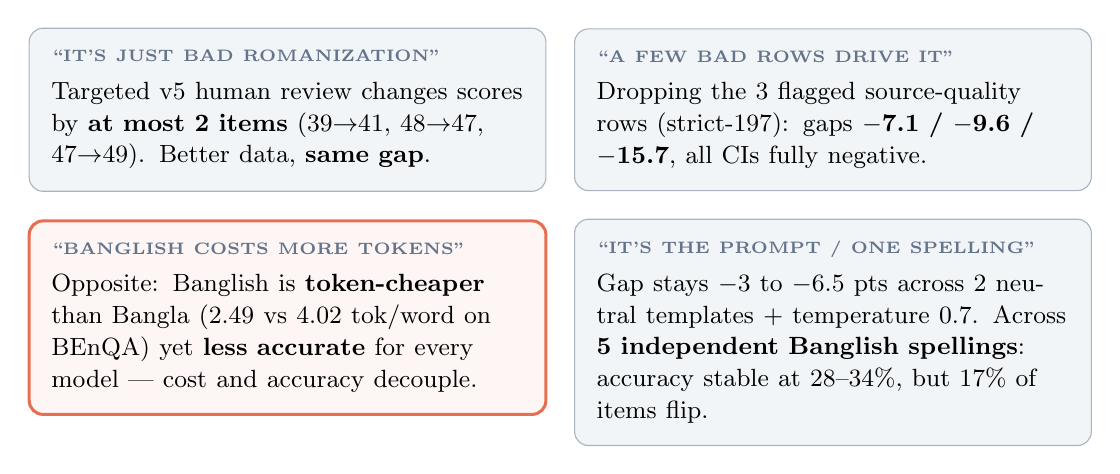
\begin{tikzpicture}[every node/.style={rounded corners=5pt,inner sep=8pt,text width=6.0cm},
                      node distance=0.3cm]
    \node[draw=cMuted!55,fill=cBg] (q1) at (0,0) {%
      \kicker{``It's just bad romanization''}
      \vspace*{2pt}
      {\fontsize{8.6}{11.5}\selectfont Targeted v5 human review changes scores by
       \textbf{at most 2 items} (39$\to$41, 48$\to$47, 47$\to$49). Better data,
       \textbf{same gap}.\par}};
    \node[draw=cMuted!55,fill=cBg,right=0.35cm of q1] (q2) {%
      \kicker{``A few bad rows drive it''}
      \vspace*{2pt}
      {\fontsize{8.6}{11.5}\selectfont Dropping the 3 flagged source-quality rows
       (strict-197): gaps \textbf{$-$7.1 / $-$9.6 / $-$15.7}, all CIs fully
       negative.\par}};
    \node[draw=cBanglish,line width=1.1pt,fill=cBanglish!6,below=0.35cm of q1] (q3) {%
      \kicker{``Banglish costs more tokens''}
      \vspace*{2pt}
      {\fontsize{8.6}{11.5}\selectfont Opposite: Banglish is \textbf{token-cheaper}
       than Bangla (2.49 vs 4.02 tok/word on BEnQA) yet \textbf{less accurate} for
       every model --- cost and accuracy decouple.\par}};
    \node[draw=cMuted!55,fill=cBg,below=0.35cm of q2] (q4) {%
      \kicker{``It's the prompt / one spelling''}
      \vspace*{2pt}
      {\fontsize{8.6}{11.5}\selectfont Gap stays $-$3 to $-$6.5 pts across 2 neutral
       templates + temperature 0.7. Across \textbf{5 independent Banglish spellings}:
       accuracy stable at 28--34\%, but 17\% of items flip.\par}};
  \end{tikzpicture}
  \end{center}
  \vspace{6pt}
  {\fontsize{9.5}{13}\selectfont The deficit survives every control $\Rightarrow$ it is
   \textbf{script-conditioned behavior}, consistent with damaged lexical grounding of
   romanized Bangla terms --- not an artifact of construction.\par}
\end{frame}

% =====================================================================
\section{Failure Analysis}
% =====================================================================

% 13 · RECOVERABILITY
\begin{frame}{40\% of Banglish misses are recoverable on the very same item}
  \vspace{2pt}
  \kicker{600 Qwen model-item slots on validation-200 v5}
  \vspace{8pt}
  \begin{center}
  \begin{tikzpicture}[xscale=0.0205, font=\fontsize{7.5}{9}\selectfont]
    % top bar: correct vs wrong (600 slots)
    \fill[cGood!75]  (0,0)   rectangle (137,0.78);
    \fill[cBad!75]   (137,0) rectangle (600,0.78);
    \node[white,font=\fontsize{8}{9}\selectfont\bfseries] at (68,0.39)  {correct 137};
    \node[white,font=\fontsize{8}{9}\selectfont\bfseries] at (368,0.39) {reviewed Banglish wrong: 463 / 600};
    % connectors
    \draw[cMuted!70,dashed] (137,0) -- (137,-0.62);
    \draw[cMuted!70,dashed] (600,0) -- (600,-0.62);
    % bottom bar: decomposition of 463 (origin at 137)
    \fill[cBangla!85] (137,-1.4)  rectangle (165,-0.62);
    \fill[cEnglish!85](165,-1.4)  rectangle (246,-0.62);
    \fill[cBoth!85]   (246,-1.4)  rectangle (322,-0.62);
    \fill[cHard!85]   (322,-1.4)  rectangle (600,-0.62);
    \node[white,font=\fontsize{7.5}{9}\selectfont\bfseries] at (205.5,-1.01) {EN-only 81};
    \node[white,font=\fontsize{7.5}{9}\selectfont\bfseries] at (284,-1.01)  {both 76};
    \node[white,font=\fontsize{7.5}{9}\selectfont\bfseries] at (461,-1.01)  {all-script hard 278};
    \node[anchor=east,cBangla!40!cInk] at (132,-1.78) {Bangla-only 28};
    \draw[cBangla!60] (151,-1.4) -- (151,-1.66) -- (135,-1.78);
    % recoverable brace
    \draw[decorate,decoration={brace,mirror,amplitude=5pt},cBanglish,line width=1pt]
      (137,-1.52) -- (322,-1.52);
    \node[cBanglish!80!cInk,font=\fontsize{8.5}{10}\selectfont\bfseries,anchor=north] at (229.5,-1.82)
      {recoverable: 185 / 463 (40\%)};
  \end{tikzpicture}
  \end{center}
  \vspace{10pt}
  \begin{itemize}
    \item These 185 misses are answered correctly by the \textbf{same model} when the
          \textbf{same item} is shown in Bangla or English $\to$ failures introduced by
          the \emph{script}, not item difficulty (55.2\% of BEnQA misses recoverable).
    \item Not absolute: 20/600 slots succeed \emph{only} in Banglish --- the claim is
          aggregate and paired, ``systematically less reliable,'' not ``always worse.''
  \end{itemize}
\end{frame}

% 14 · ERROR TAXONOMY
\begin{frame}{Why Banglish fails: no single fix will close the gap}
  \vspace{2pt}
  \begin{columns}[T]
    \column{0.50\textwidth}
      \kicker{Taxonomy of 164 recoverable BEnQA misses}
      \vspace{4pt}
      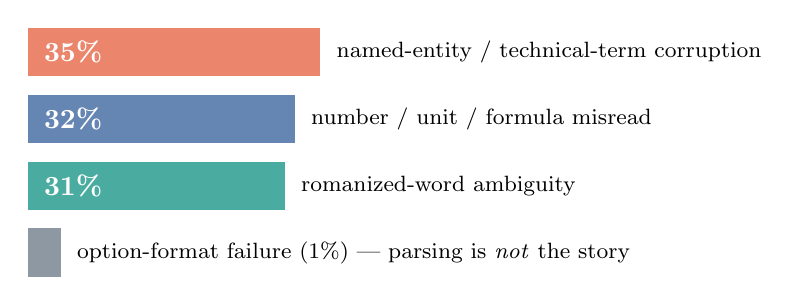
\begin{tikzpicture}[xscale=0.105, font=\fontsize{7.8}{9}\selectfont]
        \fill[cBanglish!85] (0,0)    rectangle (35.4,0.62);
        \fill[cEnglish!85]  (0,-0.85) rectangle (32.3,-0.23);
        \fill[cBangla!85]   (0,-1.70) rectangle (31.1,-1.08);
        \fill[cHard!85]     (0,-2.55) rectangle (4.0,-1.93);
        \node[anchor=west,white,font=\bfseries] at (0.8,0.31)   {35\%};
        \node[anchor=west,white,font=\bfseries] at (0.8,-0.54)  {32\%};
        \node[anchor=west,white,font=\bfseries] at (0.8,-1.39)  {31\%};
        \node[anchor=west] at (36.2,0.31)  {named-entity / technical-term corruption};
        \node[anchor=west] at (33.1,-0.54) {number / unit / formula misread};
        \node[anchor=west] at (31.9,-1.39) {romanized-word ambiguity};
        \node[anchor=west] at (4.8,-2.24)  {option-format failure (1\%) --- parsing is \emph{not} the story};
      \end{tikzpicture}
      \vspace{8pt}
      {\fontsize{8.7}{12}\selectfont Three near-balanced semantic failure modes ---
       the model loses its grip on \textbf{romanized scientific vocabulary},
       \textbf{mixed numeric context}, and \textbf{ambiguous Latin spellings}.\par}
    \column{0.47\textwidth}
      \kicker{A recoverable miss, concretely}
      \vspace{4pt}
      \begin{tikzpicture}
        \node[draw=cMuted!55,fill=cBg,rounded corners=5pt,inner sep=8pt,text width=5.7cm]{%
          {\fontsize{8.3}{11.5}\selectfont
           \textbf{benqa\_10th-Biology\_0128} --- options:\par
           \vspace*{2pt}
           \texttt{lyakotik esid · glukoj ·}\par
           \texttt{oksalo asitik esid · glisarik esid}\par
           \vspace*{4pt}
           (lactic acid, glucose, oxaloacetic acid, glyceric acid)\par
           \vspace*{5pt}
           Qwen2.5-3B: \c